% Based on:
% [1] Multics Security Evaluation: Vulnerability analysis II
% Paul A. Karger (2nd Lt, USAF)
% Roger R. Schell (Major, USAF)

% [2] A brief description of privacy measures in the Multics operating system
% Edward L. Glaser (MIT, Project MAC)

% [3] Protection and control of information sharing in Multics
% Jerome H. Saltzer (MIT, Project MAC)

% # --------------------------------------------------------------------------------- #

\section{Design Principles}
\textbf{
Design principles and overview of Security controls (section 3) are described in \textit{Protection and the control of information sharing in multics}
by J.H. Saltzer} \cite{protectionSaltzer} \textbf{and briefly by E.L. Glaser} \cite{protectionGlaser}.

\begin{enumerate}
    \item Every designer should know and understand the protection objectives of the system.
     There are many points at which \textit{"I don't care"} decision can be a breaking point 
     of internal security measurements. By keeping all designers aware of the protection objectives, 
     the decisions are more likely to be made correctly.
     
     \item Keep the design as \textit{simple} and as \textit{small} as possible. Design and 
     implementation errors which result in unwanted access paths will not be immediately noticed during 
     routine use. Therefore, techniques such as complete, \textit{line-by-line} auditing of the 
     protection mechanisms are necessary, that's the reason why small and simple design is 
     essential.

     \item Protection mechanism should be based on \textit{permission} rather than exclusion. 
     The principle means that the default situation is \textit{lack of access}, and the protection 
     scheme provides selective permission for specific purpose.

     \item Every access to every object must be checked for authority.
     
     \item The design is not secret. The mechanism do not depend on the \textit{ignorance of potential 
     attackers}, but rather on possession of specific, more easily protected, protection keys or 
     passwords. 

     \item The principle of least privilege. Every program and every privileged user of the system 
     should operate using the least amount of privilege necessary to complete the job.

     \item Make sure that the design encourages correct behaviour in the user, operators and 
     administrators of the system. It is essential that human interface be designed for naturalness, 
     ease of use and simplicity, so that user will routinely and automatically \textit{apply the 
     protection mechanisms}.

     \item Provide the option of complete decentralization of the administration of protection 
     specifications. If the system design forces all administrative decisions to be set by a single 
     administrator, that administrator quickly becomes a \textit{bottleneck}. which could result in users 
     begin adopting habits which bypass the administrator.

     \item The system provides a complete set of tools, so that a user without exercising special 
     privileges, may construct a \textit{protected subsystem}, which is a collection of programs 
     and data with the property that the data may be accessed only by programs in the subsystem, and 
     the programs may be entered only at designated entry points.
\end{enumerate}


\section{Security Controls}


\subsection{Access Control List}

The central fixture of Multics is an organized information storage system which provides reliability and 
protection from unauthorized information release. All use of information in the storage system is implemented 
by mapping the information into the virtual memory of some process. 

Storage is logically organized in separately 
named data storage segments, each which contains up to 262144 36-bit words. A segment is the cataloguing unit of 
the storage system.

Segments in Multics are stored in a hierarchy of director(Because of endless and penetrable checking of input arguments).\textit{Directory} is a special type of of
segment that is not directly accessible to the users.
Directory stores names and other information about underlying segments and directories.
Each segment and directory has an \textit{Access control list} (ACL) in its parent directory entry
\textit{who} may \textit{read}, \textit{write} or \textit{execute} (also known as 'r-w-x') the segment or obtain 
\textit{status} of, \textit{modify} entries line or \textit{append} entries on directory (also known as 's-m-a').
The ACL consists of three partitions (can be seen in \textit{Figure \ref{fig:descriptor}}):
\begin{enumerate}
    \item Every individual user of system in a separate access control group by himself with his \textit{personal name}.
    \item Sets of users in groups who cooperate in some activity, called \textit{projects}. One person may be a member of 
    several projects.
    \item  The third partition allows an individual user to create his own, named protection compartments (directories).
\end{enumerate}

For example:
User Mike in Project Compiler has all rights to read-write-execute
\begin{lstlisting}
    Mike.Compiler.x     (rwx)
\end{lstlisting}

Also \textit{asterix (*)} to grant access to \textit{all}.
User Mike in all associated project, thus directories has read-write privilege.
\begin{lstlisting}
    Mike.*.*            (rw)
\end{lstlisting}
In order to access file/directory, the ring 0 (rings mechanism is in greater details described in section cislo.cislo) 
software compares the ID of user with access control list entries.

User identification is established when user sings on to the Multics and it is stored in the Process Data 
Segment (PDS), which is accessible only in ring 0 or in Master mode - \textit{so that user cannot modify the
process data segment} and grant access anywhere on the system.

\begin{figure}
    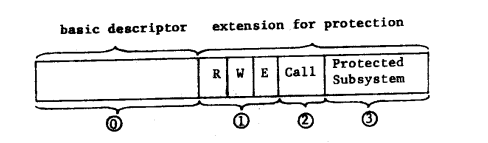
\includegraphics[scale=0.55]{images/descriptor.png}
    \caption{Multics descriptor \cite{protectionSaltzer}}
    \label{fig:descriptor}
\end{figure}

\subsection{Authentication of users}

Whole process of access control lists, access modes, protected subsystems and hierarchical control depends on an 
accurate principal identifier being associated with every process. Accuracy of the identification depends on 
authentication of the user's claimed identity.

Every user is \textit{registered} with \textit{unique name} (convention: last name, plus one or two initials) 
associated with a \textit{password} of up to eight ASCII characters. Also as another measurement, the user may 
(after authenticating) change his password at any time.

When user types a password it is \textit{enciphered} and compared with the stored enciphered version for validity.
All passwords on system are stored in non-invertible cipher (one-way encryption) form, which also acts as additional 
security in case of system dump. 

Plain text passwords are stored \textit{nowhere} on the system. As a result, passwords 
are not routinely know by any system administrator or project administrators.

Additional feature of Multics system password mechanism is that, when user is requested to give his password, the printer 
on his terminal is \textit{turned off}.(Because of endless and penetrable checking of input arguments).


Each login and logout is carefully audited to check for attempts to guess a valid password for a certain user. 
If a user provides incorrect password, the event of an \textit{incorrect login attempt} is noted in \textit{
threat-monitoring log}, and user is permitted to try again, up to ten-times at which point the telephone or network 
connection is broken by the system.

In addition each user is informed of the \textit{date}, \textit{time} and \textit{terminal identification} of last
login to detect past compromises of the users \textit{access rights}, also user is told the number of times his password 
has been given incorrectly since its last correct use in his greeting message. 


\subsection{Primary Memory Protection}

The virtual address space of a Multics process is implemented with an \textit{array of descriptors}, called 
a \textit{descriptor segment}. Every reference to the virtual memory specifies both, segment number (index) and a 
word number within the segment.

The reason why the protection information is associated with the addressing descriptor rather than data itself is, 
in \textit{multiprocessor system} such as Multics, two same processes may be executing at a same time, so single 
protection specification associated with the data is not sufficient.

\begin{enumerate}
    \item Physical address and size of the segment based on this descriptor.
    \item Bits separately controlling permission (read-write-execute).
    \item Control of permission to enter a protected subsystem which has entry points in the segment.
    \item Controls on which protected subsystems may use this descriptor.
\end{enumerate}

Another feature of the descriptors used in Multics is implemented inside the \textit{second} and \textit{third} part of descriptor, 
which can be seen on \textit{Figure} \ref{fig:descriptor}, together they allow hardware enforcement of protected subsystems, 
which are intended to be used only by calls to \textit{designated entry points}, know as \textit{gates}. As a result of this, 
it is possible to construct proprietary programs which cannot be read. They return only statistics rather than raw data.

\textit{Protected subsystems} are formed by using the \textit{third field} of the descriptor extension. Multics force a 
\textit{hierarchical} constraint on all subsystems within a single process. Each subsystem is assigned a number between 
\textbf{0} and \textbf{7}. This scheme is also called \textit{the ring mechanism} or \textit{the rings of protection}. 
The protection rings are defined in the way:
\textit{The higher numbered rings having less privilege than lower numbered rings, and ring 0
containing 'hardcore' supervisor}. Therefore, each subsystem is permitted to use all of those descriptors containing 
protected subsystem numbers greater or equal to its own.

The descriptors are adjusted to provide \textit{only} the amount of access required by the \textit{supervisor} in direct 
harmony of \textit{Design principal number 6}. These mechanism do not prohibit the supervisor from making full use of hardware, 
rather than protection against accidental/exploitation overuse of supervisor privileges.

\subsection{Master Mode}

The convention around protecting \textit{master mode software}, was specified as the master mode procedures
were not to be used outside ring 0. Convention had been defined as of "\textit{each master mode procedure must 
have a master mode pseudo-operation code assembled into location 0}".
The master mode pseudo-operation generates code to test an index register for a value corresponding to an 
entry point in the segment. If the index register is invalid, the master mode pseudo-operation saves the
registers for debugging and shuts the system down.

\subsection{Software Maintenance Procedure}

The system is initialized from a magnetic tape which contains copies of every program residing in the \textit{most protected 
area}. The maintenance of the \textit{Multics software} had been carried out \textbf{online} on a \textit{dial-up 
Multics facility}. A programmer prepared (and debugs) his software for installation, then submits his
software to a \textit{library installer} who copied and recompiled the source code in a \textit{protected 
directory}. 
The software prior installing into the system source and object libraries is checked by library installer.
Ring 0 software is stored on a \textit{system tape} that is reloaded into the system each time it is brought up.
(New system tapes are generated from online copies of the ring 0 software).
The system libraries had been protected against modification by access control list mechanism. In addition 
the library installers had been periodically checked of last modification of all segments in the library to
detect unauthorized modifications.